\documentclass{beamer}
\usepackage{xcolor}
\usepackage{natbib} % package to organize literature
\usepackage{multicol}
\usepackage{booktabs}
\usepackage{wasysym} % additional symbols
\usepackage{graphicx} % to include graphics, gifs
\usepackage{color} % add colored text
\usepackage{lmodern} % to fix font size error, might be problematic with math symbols
\usepackage{array}
\usepackage{tikz}
\usepackage{arydshln} % dashed lines

\usetheme{Frankfurt}
\usecolortheme{beaver}
\setbeamertemplate{footline}
{
  \leavevmode%
  \hbox{%
  \begin{beamercolorbox}[wd=.3\paperwidth,ht=2.25ex,dp=1ex,center]{author in head/foot}%
    \usebeamerfont{author in head/foot}\insertshortauthor \hspace{1em} (\insertshortinstitute)
  \end{beamercolorbox}%
  \begin{beamercolorbox}[wd=.4\paperwidth,ht=2.25ex,dp=1ex,center]{title in head/foot}%
    \usebeamerfont{title in head/foot}\insertshorttitle
  \end{beamercolorbox}%
  \begin{beamercolorbox}[wd=.3\paperwidth,ht=2.25ex,dp=1ex,right]{author in head/foot}%
    \usebeamerfont{author in head/foot}\insertdate \hspace{2em}
    \insertframenumber{} / \inserttotalframenumber\hspace*{1em}
  \end{beamercolorbox}}%
  \vskip0pt%
}
%\definecolor{beamer@sbred}{rgb}{0.65,0.15,0.18}
\definecolor{beamer@sbred}{rgb}{0.22,0.22,0.66}
\setbeamercolor{title}{fg=beamer@sbred,bg=black!5}
\setbeamercolor{structure}{fg=beamer@sbred}
\setbeamercolor{frametitle}{fg=beamer@sbred}
\setbeamercolor{palette primary}{fg=beamer@sbred,bg=black!10}
\setbeamercolor{palette secondary}{fg=beamer@sbred}
\setbeamercolor{palette tertiary}{bg=beamer@sbred}
\setbeamercolor{palette quaternary}{fg=white,bg=beamer@sbred}
\setbeamertemplate{itemize items}[default]
\setbeamertemplate{enumerate items}[default]
\setbeamersize{text margin left=1em,text margin right=1em}
\DeclareTextFontCommand{\emph}{\color{beamer@sbred}}

\setbeamercolor*{block title example}{fg= white, bg= beamer@sbred!90}
\setbeamercolor*{block body example}{fg= black, bg= beamer@sbred!10}

% remove institution parentheses in foot info line
    \defbeamertemplate*{footline}{my infolines theme}
    {
      \leavevmode%
      \hbox{%
      \begin{beamercolorbox}[wd=.333333\paperwidth,ht=2.25ex,dp=1ex,center]{author in head/foot}%
        \usebeamerfont{author in head/foot}\insertshortauthor~~\insertshortinstitute
      \end{beamercolorbox}%
      \begin{beamercolorbox}[wd=.333333\paperwidth,ht=2.25ex,dp=1ex,center]{title in head/foot}%
        \usebeamerfont{title in head/foot}\insertshorttitle
      \end{beamercolorbox}%
      \begin{beamercolorbox}[wd=.333333\paperwidth,ht=2.25ex,dp=1ex,right]{date in head/foot}%
        \usebeamerfont{date in head/foot}\insertshortdate{}\hspace*{2em}
        \insertframenumber{} / \inserttotalframenumber\hspace*{2ex}
      \end{beamercolorbox}}%
      \vskip0pt%
    }

% settings for tikz
\usetikzlibrary{arrows,positioning} 
\tikzset{
    %Define standard arrow tip
    >=stealth',
    %Define style for boxes
    punkt/.style={
           rectangle,
           rounded corners,
           draw=black, very thick,
           text width=6.5em,
           minimum height=2em,
           text centered},
    % Define arrow style
    pil/.style={
           ->,
           thick,
           shorten <=2pt,
           shorten >=2pt,}
}

\author[Patrick Kraft (Stony Brook University)]{Patrick W. Kraft}
\institute[]{75\textsuperscript{th} MPSA Annual Conference, Chicago, Il}
\title[Women Also Know Stuff]{Women Also Know Stuff\\
{\large Challenging the Gender Gap in Political Sophistication}}
\date{April 8\textsuperscript{th}, 2017}
\titlegraphic{\includegraphics[height=.7cm]{/data/Dropbox/Uni/Misc/Logos/logo_bk.pdf}}

\begin{document}
\frame{\titlepage}
%\footnotesize


% ADD empty table
\section{Introduction}
\subsection{}
\begin{frame}%[allowframebreaks]
\frametitle{Quiz: Who scores higher on political knowledge?}
\begin{table}[ht]\tiny\centering
\begin{tabular}{l|p{4.5cm}|p{4.5cm}}
   \toprule
%  & Low Sophistication Response & High Sophistication Response \\ 
    & \textbf{Respondent A} & \textbf{Respondent B} \\ 
   \midrule
   Obama (+) & The healthcare, keeping that and the financial aid, helping students. & I think he is honest, has good intentions. \\ \hdashline
     Obama (-) &  & I don't feel he is up for the job, he doesn't really know how to get things accomplished from idea to actual reality. \\ \hdashline
     Romney (+) &  & He comes across as an honest person and I feel that financially he would be better for the country. \\ \hdashline
     Romney (-) & By taking financial aid away from students, taking family type planing, healthcare type of help away. & I am a moderate conservative and there are some things about anti-gay rights that I don't support. \\ \hdashline
     Democrats (+) & Mostly the healthcare, mostly people do need healthcare and can't afford to pay insurance. Financial aid most people cant afford to go college. Main two things that I like is the help with education and to pay for insurance to go to doctor. & They do seem to be generally concerned with everyone, taking care of the country as a whole. \\ \hdashline
     Democrats (-) &  & They fight too much among themselves and I disagree with wealth redistribution. \\ \hdashline
     Republicans (+) &  & I agree with a lot of the conservative values and taking responsibility for one's own actions. \\ \hdashline
     Republicans (-) &  & They argue too much among themselves and don't accomplish very much. \\ 
    \bottomrule
 \end{tabular}
\end{table}
\end{frame}

\subsection{}
\begin{frame}%[allowframebreaks]
\frametitle{Introduction}
\begin{center}
\large{Both respondents scored equally on the conventional political knowledge measure in the 2012 ANES!}
\end{center}
\end{frame}
% NOTE: I want to convinvce you of two things:
% - there is meaningful variance in open-ended responses that is directly related to our conceptualization of political sophistication
% - if we use open-ended responses to measure sophistication, gender differences disappear.


\subsection{}
\begin{frame}{Data Overview}
\begin{itemize}
\item 2012 ANES
\end{itemize}
\end{frame}

\section{Validating the Measure}

\subsection{}
\begin{frame} %[allowframebreaks]
  \begin{figure}
  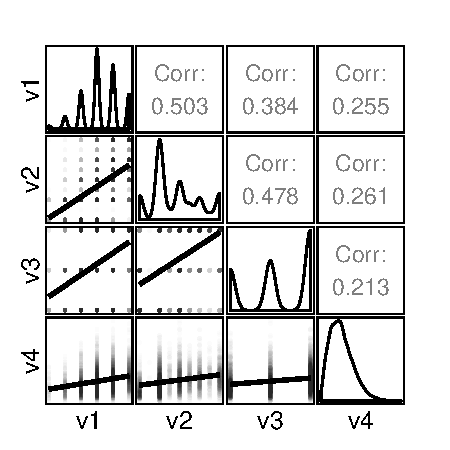
\includegraphics[height = .9\textheight]{../fig/corplot.pdf}
  \end{figure}
\end{frame}

\section{Validating the Measure}

\subsection{}
\begin{frame} %[allowframebreaks]
  \frametitle{Topic Proportions}
  \begin{figure}
  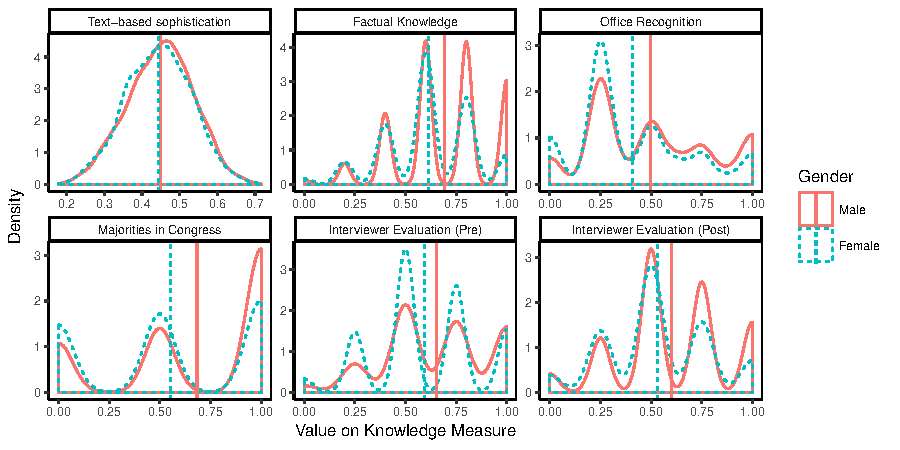
\includegraphics[width = \textwidth]{../fig/densities.pdf}
  \end{figure}
\end{frame}


\section{Conclusion}
\subsection{}
\begin{frame}%[allowframebreaks]
  \frametitle{Conclusion}
  \begin{itemize}
\item Something about political \emph{knowledge}
\item We can measure interesting stuff when looking at open-ended items...
\item This is kind of consistent with Lupia's competence argument but now we do not assume what individuals have to know.
\end{itemize}
\end{frame}

\subsection{}
\begin{frame}%[allowframebreaks]
  \begin{center}
  \large{Thank you very much for your attention!}\\ \vspace{2em}
  Manuscript and code available at:\\
  \emph{\texttt{https://github.com/pwkraft/knowledge}}\\ \vspace{2em}
  Comments, questions?\\
  \emph{\texttt{patrick.kraft@stonybrook.edu}}
  \end{center}
\end{frame}

\subsection{}
\begin{frame}
  \frametitle{References}
  \def\newblock{\hskip .11em plus .33em minus .07em}
  %\nocite{*}
  \begin{scriptsize}
    \bibliographystyle{../paper/apsr2006}
    \bibliography{../paper/JBRReferences.bib}
  \end{scriptsize}
\end{frame}

\end{document}